\chapter{Software Development}
\label{chap:software_analysis}
\thispagestyle{empty}

The subsequent chapter focuses on the software developed to evaluate the interferometric signals.
The primary objective of the software was to provide an independent measurement of stage displacement based on interferometric fringe counting and directly comparing this value with the displacement reported by the translation stage controller. For this purpose, three software implementations were developed: one for camera-based fringe counting, one for photodiode-based fringe counting, and one for evaluating the quadrature homodyne interferometer.

\section{Software for Fringe detection with the Camera}
Several functional requirements were identified before development began.

First, the software had to continuously acquire images from the camera while maintaining a responsive user interface. Second, it had to reliably detect and count interference fringes in real time despite fluctuations in illumination and environmental noise. Third, direct control of the electronic translation stage was required, including both relative and absolute positioning commands.

Finally, the measured interferometric displacement had to be continuously compared with the displacement reported by the stage controller in order to evaluate positioning accuracy.

The software was implemented in Python and organized into three main components: a graphical user interface, a camera handling module, and a translation stage control module.

\subsection{Graphical User Interface}

The graphical user interface was implemented using the \texttt{CustomTkinter} library. It provides all user interaction functions, including starting and stopping measurements, entering the laser wavelength, controlling stage motion and displaying measurement results.

A screenshot of the user interface implementation is shown in Figure~\ref{fig:software_gui}.

\begin{figure}[htbp]
    \centering
    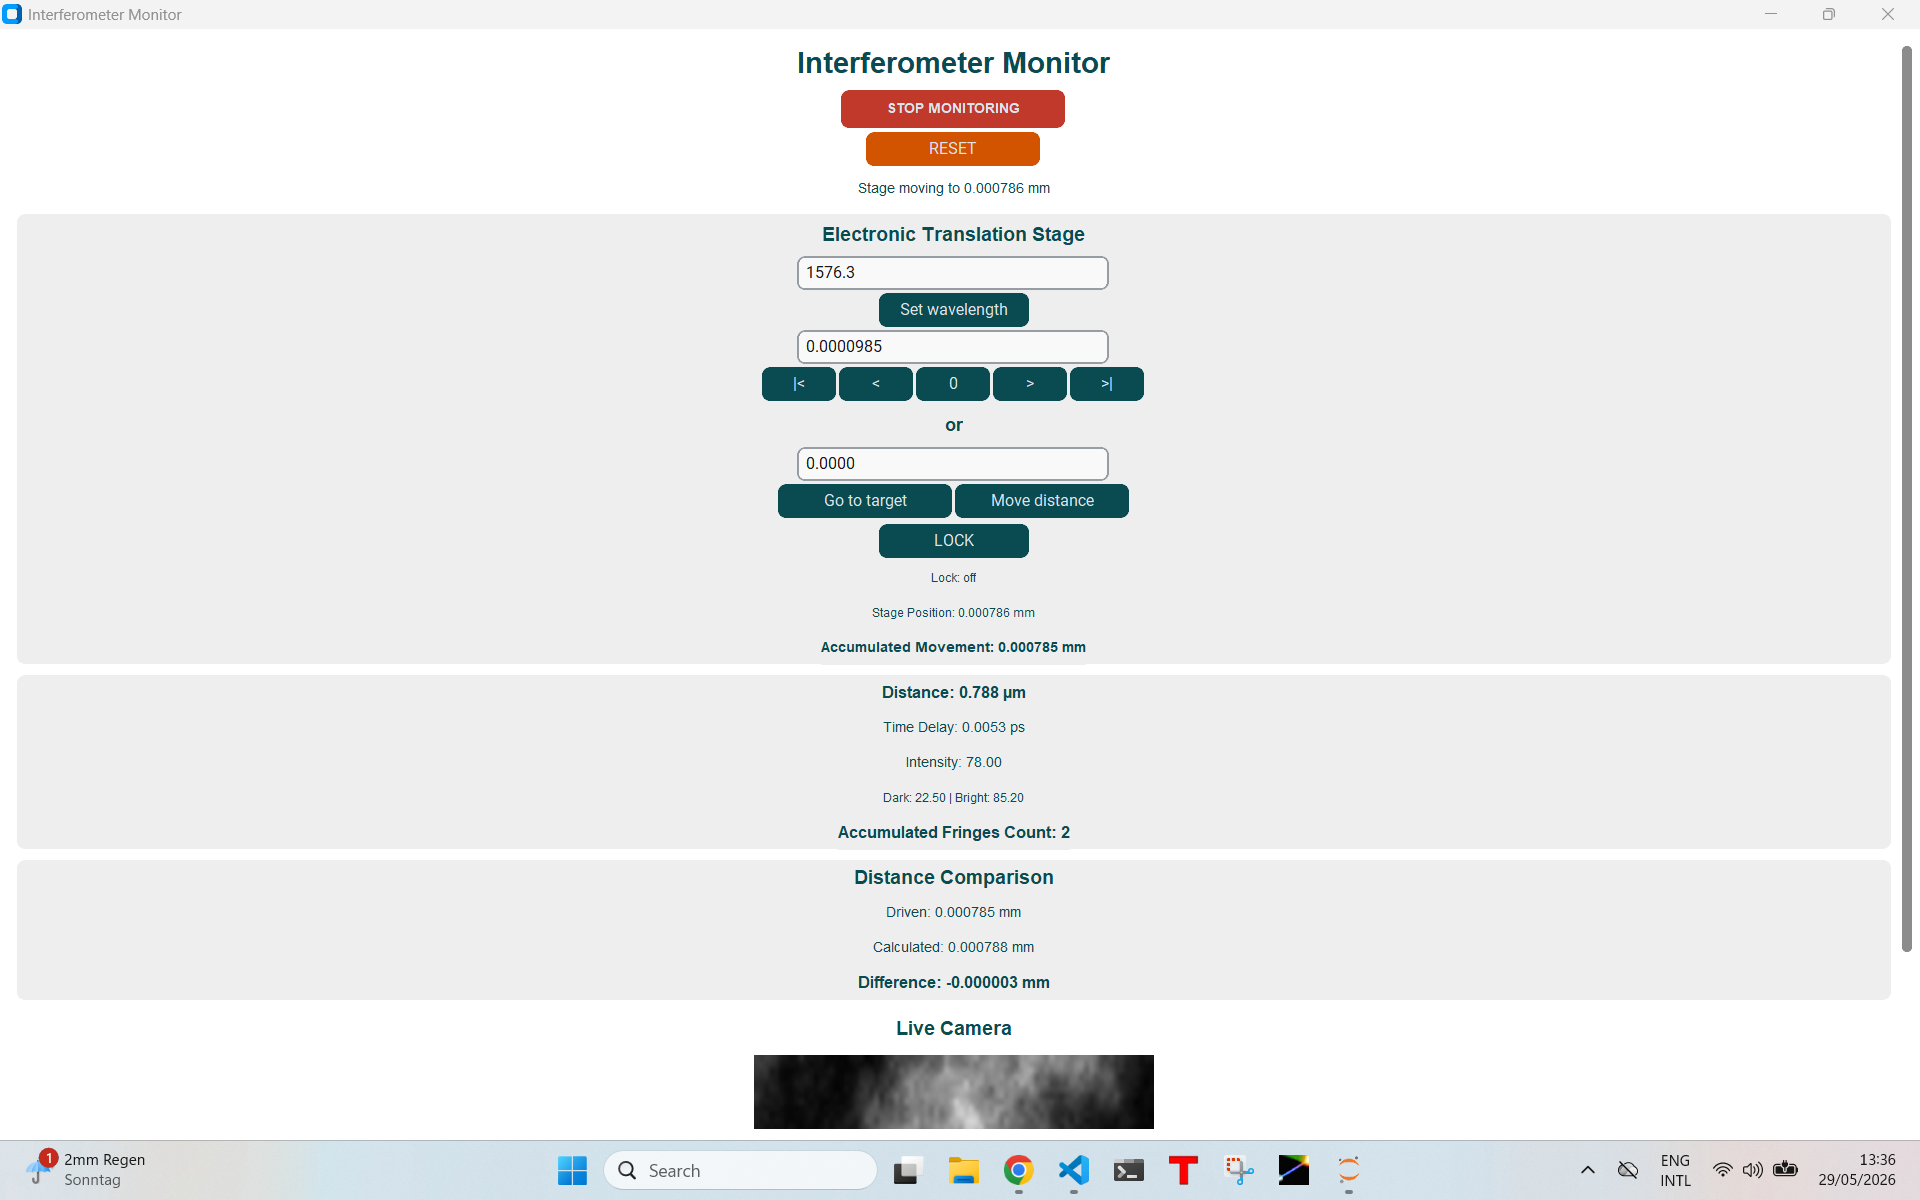
\includegraphics[width=\linewidth]{figures/interferometerwmeasurement3.png}
    \caption{Graphical user interface of the developed Camera monitoring software.}
    \label{fig:software_gui}
\end{figure}

The interface displays the current fringe intensity, accumulated fringe count, interferometrically measured displacement, optical time delay, stage position, and the difference between commanded and measured displacement. A live image of the camera is also displayed to assist with alignment and monitoring.

\subsection{Camera Handler}

Communication with the Thorlabs camera was implemented in a dedicated \texttt{Camera\-Handler} module. This module is responsible for loading the required camera drivers, acquiring images, extracting the fringe intensity from each frame, and providing image data to the graphical user interface.

Separating camera functionality from the main application simplified maintenance and reduced the complexity of the graphical user interface code.

\subsection{Stage Handler}

Control of the electronic translation stage was implemented in a separate \texttt{StageHandler} module. This module handles all communication with the stage hardware, including position queries, absolute movements, relative movements and motion limits.

\subsection{Automatic Calibration}

Reliable fringe detection requires accurate identification of bright and dark interference states. Since the observed intensity range depends on camera exposure, optical alignment, and environmental conditions, fixed threshold values are generally unsuitable.

To overcome this limitation, an automatic calibration procedure was implemented. Whenever monitoring is started, the software enters a calibration phase lasting five seconds.

During this period, the translation stage performs a predefined forward and backward motion of about one fringe distance while the software continuously records the measured fringe intensities. The resulting intensity values are stored and used to determine the minimum intensity \(I_{\min}\) and the maximum intensity \(I_{\max}\).

The dark threshold is then calculated as

\[
I_{\mathrm{dark}}
=
I_{\min}
+
0.125
\left(
I_{\max}-I_{\min}
\right),
\]

while the bright threshold is determined by

\[
I_{\mathrm{bright}}
=
I_{\max}
-
0.40
\left(
I_{\max}-I_{\min}
\right).
\]

These parameters were determined experimentally and were found to provide reliable fringe detection under the investigated operating conditions. The dark threshold was set close to \(I_{\min}\), resulting in a conservative classification that accepts only clearly defined intensity minima. The bright threshold was set farther below \(I_{\max}\), because the measured bright fringes did not always reach the absolute maximum intensity. 

After calibration, the stage automatically returns to its reference position and all measurement counters are reset. To prevent accidental user interaction during this transition, all control buttons remain disabled for an additional two seconds.

As a fallback option, manually defined threshold values can also be used if automatic calibration fails.

\subsubsection{Fringe Detection Algorithm}

The core functionality of the software is the detection and counting of interference fringes from the camera signal.

\subsubsection{Threshold-Based Detection}

The measured fringe intensity is continuously compared with the calibrated dark and bright thresholds in a fixed region of interest in the camera signal. Whenever the intensity falls below the dark threshold, the software identifies the current fringe state as dark. Similarly, intensities above the bright threshold are classified as bright.

Using two separate thresholds reduces sensitivity to small fluctuations near the transition region.

\subsubsection{Moving Average Filtering}

Camera noise and short-term intensity fluctuations may cause individual frames to be incorrectly classified. To suppress such disturbances, the software applies a moving average filter to the most recent five intensity measurements.

The filtered intensity is given by

\[
I_{\mathrm{filtered}}
=
\frac{1}{N}
\sum_{i=1}^{N}
I_i,
\]

where \(N\) is the number of averaged measurements and \(I_i\) represents the intensity of the \(i\)-th measurement. The filter window size is set to

\[
N = 5.
\]

This smoothing operation significantly improves detection stability without noticeably affecting response time.



\subsubsection{State Machine}

Fringe counting is implemented using a state-based approach. The software first waits until a stable dark fringe has been detected. Once this condition is satisfied, the system enters a waiting state and monitors for the appearance of a stable bright fringe.

A fringe is counted only when a confirmed bright state follows a previously confirmed dark state. After a fringe has been counted, the state machine is reset and the process begins again.

This approach prevents multiple counts from being generated by small oscillations around the threshold values.

\subsubsection{Consecutive Frame Validation}

To further improve robustness, a state transition is accepted only after multiple consecutive frames satisfy the corresponding threshold condition.

The values

\[
N_{\mathrm{dark}} = 3
\quad\text{and}\quad
N_{\mathrm{bright}} = 3
\]

were found experimentally to provide reliable operation.

Consequently, at least three consecutive dark frames are required before a dark state is accepted, and at least three consecutive bright frames are required before a bright state is accepted.

\subsubsection{Cooldown Mechanism}

The cooldown time was initially determined experimentally. For the stage velocity used during the experiment, a value of

\begin{equation}
t_{\text{cooldown}} = 80\,\mathrm{ms}
\end{equation}

was found to reliably prevent multiple counts caused by intensity fluctuations around the detection threshold.

However, a fixed cooldown time is only suitable for a limited range of stage velocities. If the user selects a higher velocity, the time between two consecutive fringes decreases. In this case, a fixed cooldown may suppress valid fringes.

Therefore, the cooldown time is calculated adaptively from the selected stage velocity. Instead of using a fixed delay, the software estimates the expected time interval between two consecutive fringes from the current velocity setting and the known laser wavelength. The experimentally determined cooldown of approximately \(80\,\mathrm{ms}\) corresponded to about one eighth of the expected fringe period at the measurement velocity used during calibration. This ratio was therefore used as the scaling factor for the adaptive implementation:

\begin{equation}
t_{\text{cooldown}}
=
\frac{T_{\text{Fringe}}}{8}.
\end{equation}

Here, \(T_{\text{Fringe}}\) denotes the velocity-dependent time between two consecutive fringes.

Thus, the cooldown time automatically decreases when the user selects a higher stage velocity and increases when a lower velocity is selected. This prevents valid fringes from being suppressed while preserving the experimentally determined relation between the cooldown time and the expected fringe period.

\subsection{Translation Stage Control}

The software provides several methods for controlling the electronic translation stage.

The user may move the stage to an absolute position, move it by a relative distance, or perform incremental movements using a configurable step size. Additional buttons allow direct movement to the minimum position, center position, or maximum position of the stage travel range.

The default step size is automatically calculated from the laser wavelength and corresponds to one quarter of the fringe distance. This allows precise positioning while ensuring that individual fringes cannot easily be skipped during motion.

All stage movements are executed in background threads to prevent the graphical user interface from becoming unresponsive during motion.

\subsection{Conversion of Fringe Count to Displacement}

The fringe count obtained from the interference signal is converted into a physical displacement using the known laser wavelength.

For a Michelson interferometer, the optical path difference changes by twice the mechanical displacement of the translation stage. Since the implemented algorithm counts transitions between dark and bright fringes, one counted fringe step corresponds to a stage displacement of

\[
d_{\mathrm{fringe}}
=
\frac{\lambda}{2}.
\]

Using the measured wavelength of the selected laser source,

\[
\lambda = 787.3\,\mathrm{nm},
\]

the corresponding displacement per counted fringe step is

\[
d_{\mathrm{fringe}}
=
0.394\,\mu\mathrm{m}.
\]

The total interferometrically measured displacement is calculated from the accumulated fringe count according to

\[
d
=
N_{\mathrm{fringe}}
\cdot
d_{\mathrm{fringe}},
\]

where \(N_{\mathrm{fringe}}\) denotes the accumulated fringe count. In addition, the software converts the measured displacement into the corresponding optical time delay:

\[
\Delta t
=
\frac{2d}{c},
\]

where \(c\) is the speed of light.

\subsection{Comparison of Stage and Interferometric Displacement}

A key objective of the developed software is to compare the displacement reported by the translation stage controller with the displacement measured interferometrically by fringe counting.

For each movement, the software continuously calculates the displacement deviation

\[
\Delta d
=
d_{\mathrm{stage}}
-
d_{\mathrm{interferometer}},
\]

where \(d_{\mathrm{stage}}\) is the displacement reported by the stage controller and \(d_{\mathrm{interferometer}}\) is the displacement determined from the fringe count.

The resulting deviation provides a direct measure of the positioning error and enables a quantitative evaluation of the accuracy and repeatability of the translation stage.

\section{Software for Fringe Detection with the Photodiode}

The software developed for the photodiode-based fringe detection follows the same general structure as the camera-based implementation described in the previous section. The graphical user interface is again implemented using the \texttt{CustomTkinter} library, while the hardware communication is separated into dedicated handler classes. Instead of processing camera images, the software now uses a \texttt{SingleDiodeHandler} class, which establishes the connection to the National Instruments data acquisition (NI-DAQ) device and continuously reads the voltage signal of the photodiode. The main application, which coordinates the user interface, the measurement process and the control of the electronic translation stage.

As with the camera software, the measurement process is executed in a separate thread. This allows the voltage acquisition, translation stage movement and graphical user interface to run simultaneously without freezing the application. During the measurement, the user interface continuously updates the measured voltage, the accumulated fringe count, the calculated optical path difference, the corresponding time delay and the current position of the translation stage.

Figure~\ref{fig:single_diode_software_gui} shows the user interface of the single-photodiode software. Because not all controls and plots fit into one visible window, the interface is shown in two parts.

\begin{figure}[htbp]
    \centering
    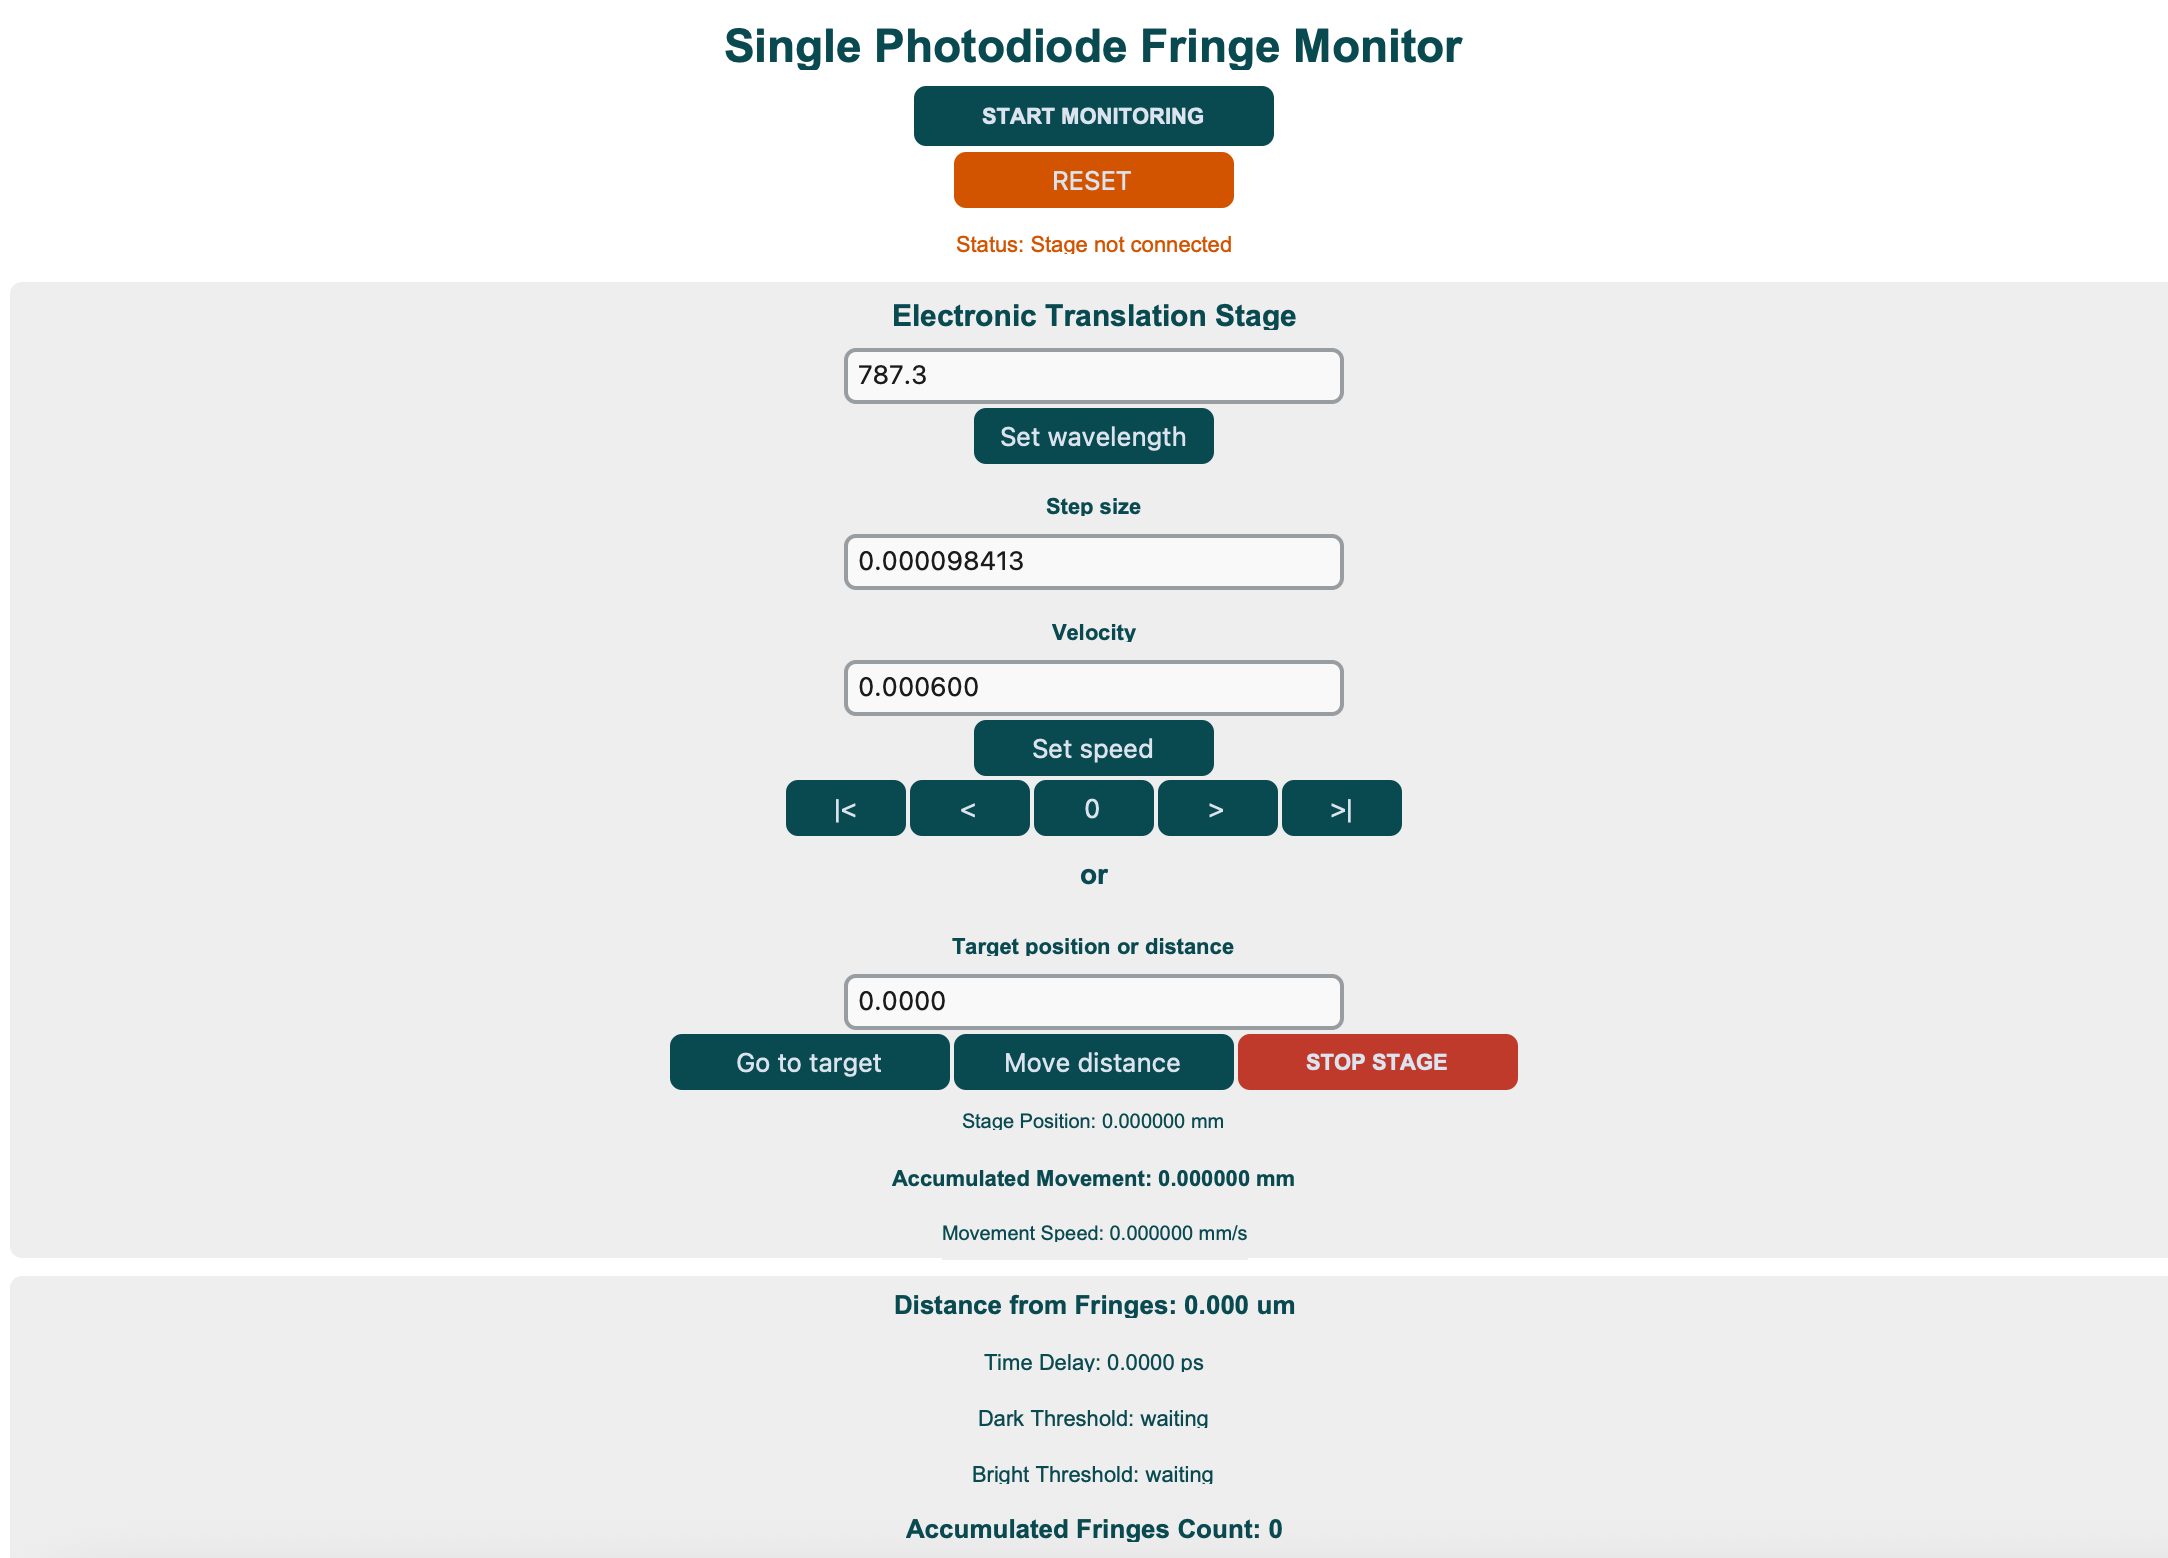
\includegraphics[width=0.92\linewidth]{figures/diodesoftwareoben.png}\par\vspace{0.5em}
    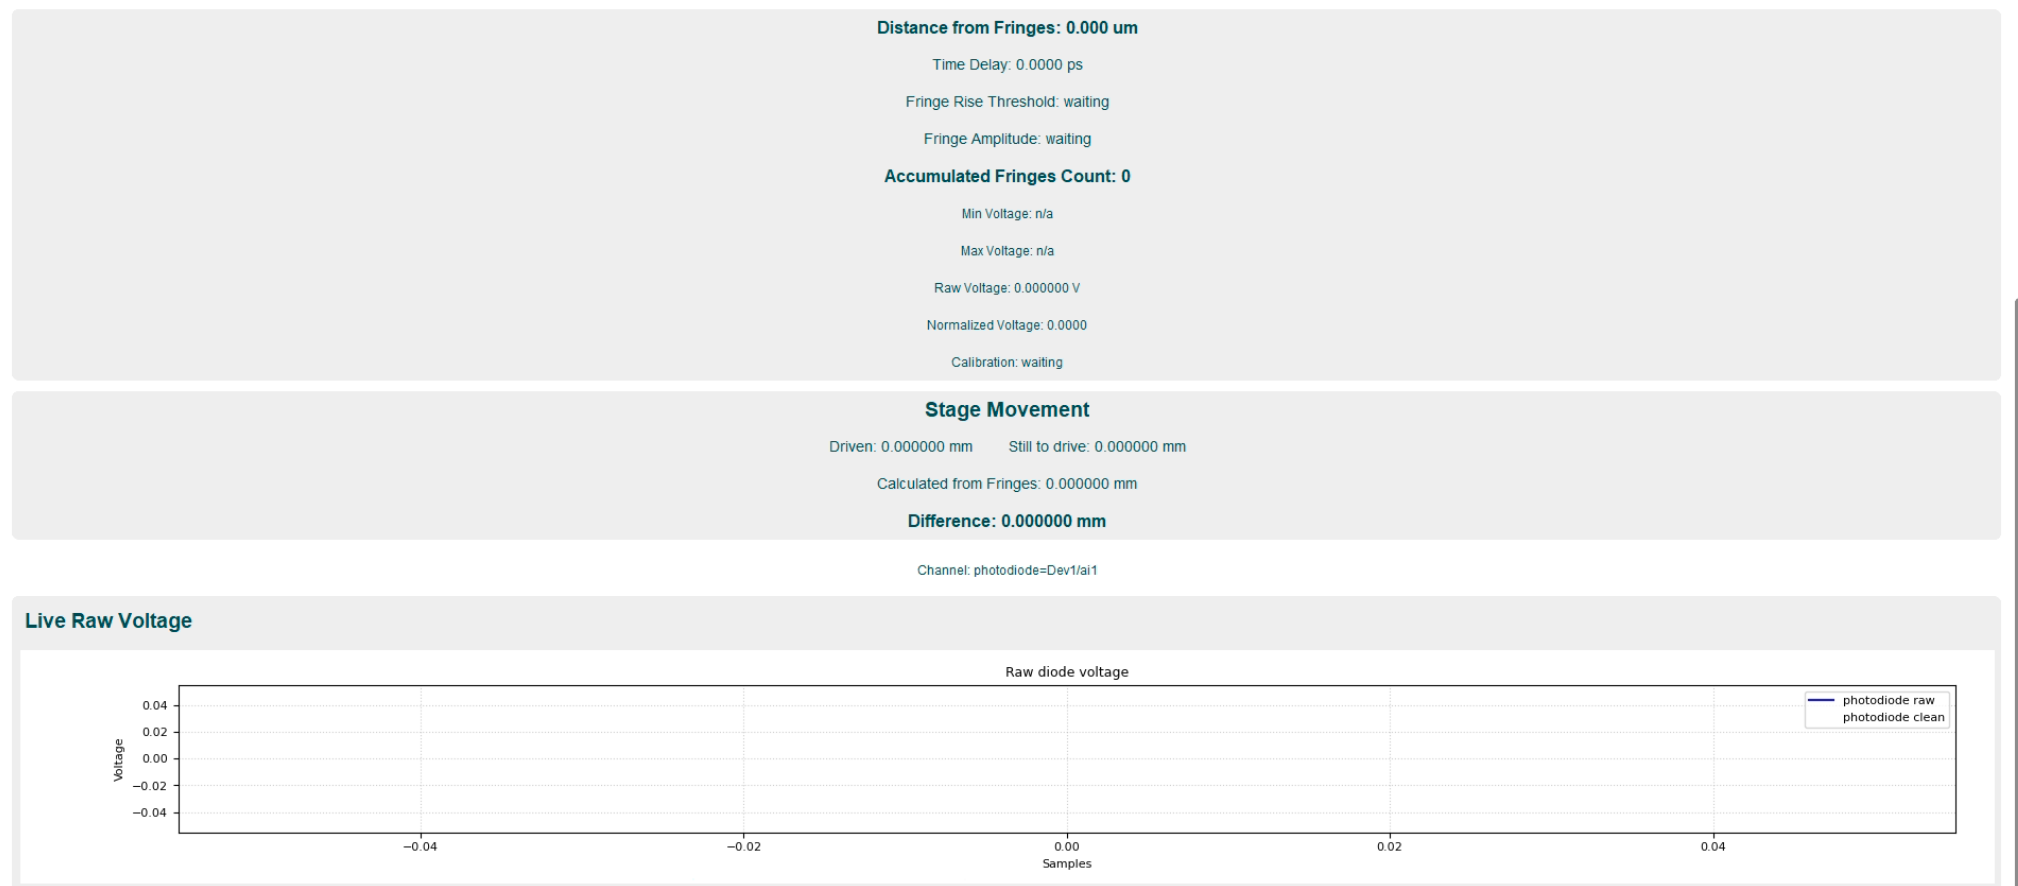
\includegraphics[width=0.92\linewidth]{figures/diodesoftwareunten.png}
    \caption{Graphical user interface of the single diode software. Top: upper part of the scrollable interface. Bottom: lower part of the interface.}
    \label{fig:single_diode_software_gui}
\end{figure}

\subsection{Measurement Procedure}

After the user starts the measurement, the software first establishes communication with the NI-DAQ device and the translation stage. Before the actual fringe detection begins, the first 200 acquired voltage samples are recorded while the translation stage remains stationary. These samples are averaged to determine the electrical baseline of the photodiode signal,

\begin{equation}
V_\mathrm{baseline}=\frac{1}{N}\sum_{i=1}^{N}V_i,
\end{equation}

with $N=200$. This baseline is then subtracted from every following measurement,

\begin{equation}
V_\mathrm{clean}=V_\mathrm{raw}-V_\mathrm{baseline},
\end{equation}

which removes the constant voltage offset and improves the signal-to-noise ratio.

The software also includes the option to use a reference photodiode. In this configuration, a small fraction of the laser beam is split off directly behind the laser output and detected by a second photodiode. The reference signal can then be used for normalization in order to compensate for slow fluctuations of the laser intensity. 

\subsection{Automatic Calibration}

Before the measurement starts, the software performs an automatic calibration equal to the one used in the Camera software. 

The photodiode signal showed noticeable fluctuations in both amplitude and offset over time. Therefore, detecting fringes by identifying local minima and maxima, as done for the camera images, did not provide reliable results. Instead, an adaptive calibration procedure was implemented.

First, the recorded calibration data are smoothed using a moving average filter to reduce high-frequency noise. Afterwards, local minima and maxima are identified from the filtered signal. From these extrema, the software estimates the fringe amplitude while automatically rejecting small extrema that originate from electrical noise. In addition, the noise level is estimated from the calibration data and used to calculate a minimum valid fringe amplitude. Only signal changes that clearly exceed this noise level are accepted as valid fringes.

Based on the measured fringe amplitude, the software automatically calculates the thresholds required for the subsequent fringe detection algorithm. Since these thresholds are determined individually for every measurement, the software adapts automatically to changing signal conditions without requiring manual parameter adjustment.

\subsection{Fringe Detection}

The implemented fringe detection algorithm is based on the measured fringe amplitude rather than on directly detecting local minima and maxima. This approach proved to be considerably more robust for the photodiode measurements, whose signal characteristics changed over time.

Before evaluating the signal, every newly acquired voltage sample is smoothed using a short moving average filter. The detection algorithm then operates as a state machine consisting of a dark state and a bright state.

Initially, the algorithm waits until the signal reaches the dark region of an interference fringe. Once this condition is fulfilled, the signal is monitored until it rises by a predefined fraction of the calibrated fringe amplitude. When this threshold is exceeded for several consecutive samples, one fringe is counted.

The control of the translation stage as well as distance calculation, cooldown period and all further calculations are identical to the Camera Software mentioned above.

Finally, the software provides the possibility to record all measured data. The recorded dataset contains the relative measurement time, the raw voltage, the baseline-corrected voltage, the accumulated fringe count, the calculated optical distance and the current position of the translation stage. After the measurement, these data can be exported as a CSV file for further analysis. A visualization of the user interface is shown in Figure~\ref{fig:single_diode_software_gui}.

\section{Software for Homodyne Quadrature Detection}

The software for homodyne quadrature detection is based on the same structure as the software presented for the single-photodiode measurements. Therefore, components such as the graphical user interface, data acquisition via the NI-DAQ device, baseline correction, data recording and the general software architecture are implemented in the same way and are not described again in detail. The main difference is that the interferometric signal is now evaluated from two photodiodes instead of only one. These two signals are phase shifted by \(90^\circ\), allowing the optical phase to be determined directly.

The analog voltages of both photodiodes are recorded simultaneously by the \texttt{NIPhotodiode\-Reader} class using two analog input channels of the NI-DAQ device. After acquisition, both signals are processed by the \texttt{HomodyneQuadrature\-Counter}. In parallel, a \texttt{SingleSignalFringe\-Counter} is executed for each signal. Its implementation is identical to the one described in the previous section and is mainly used to verify whether both photodiode signals contain visible interference fringes before the quadrature evaluation is started.

The graphical user interface of the homodyne quadrature software is shown in Figure~\ref{fig:homodyne_software_gui}. Since the interface contains more information than can be displayed in one window view, the upper and lower parts of the scrollable interface are shown separately.

\begin{figure}[htbp]
    \centering
    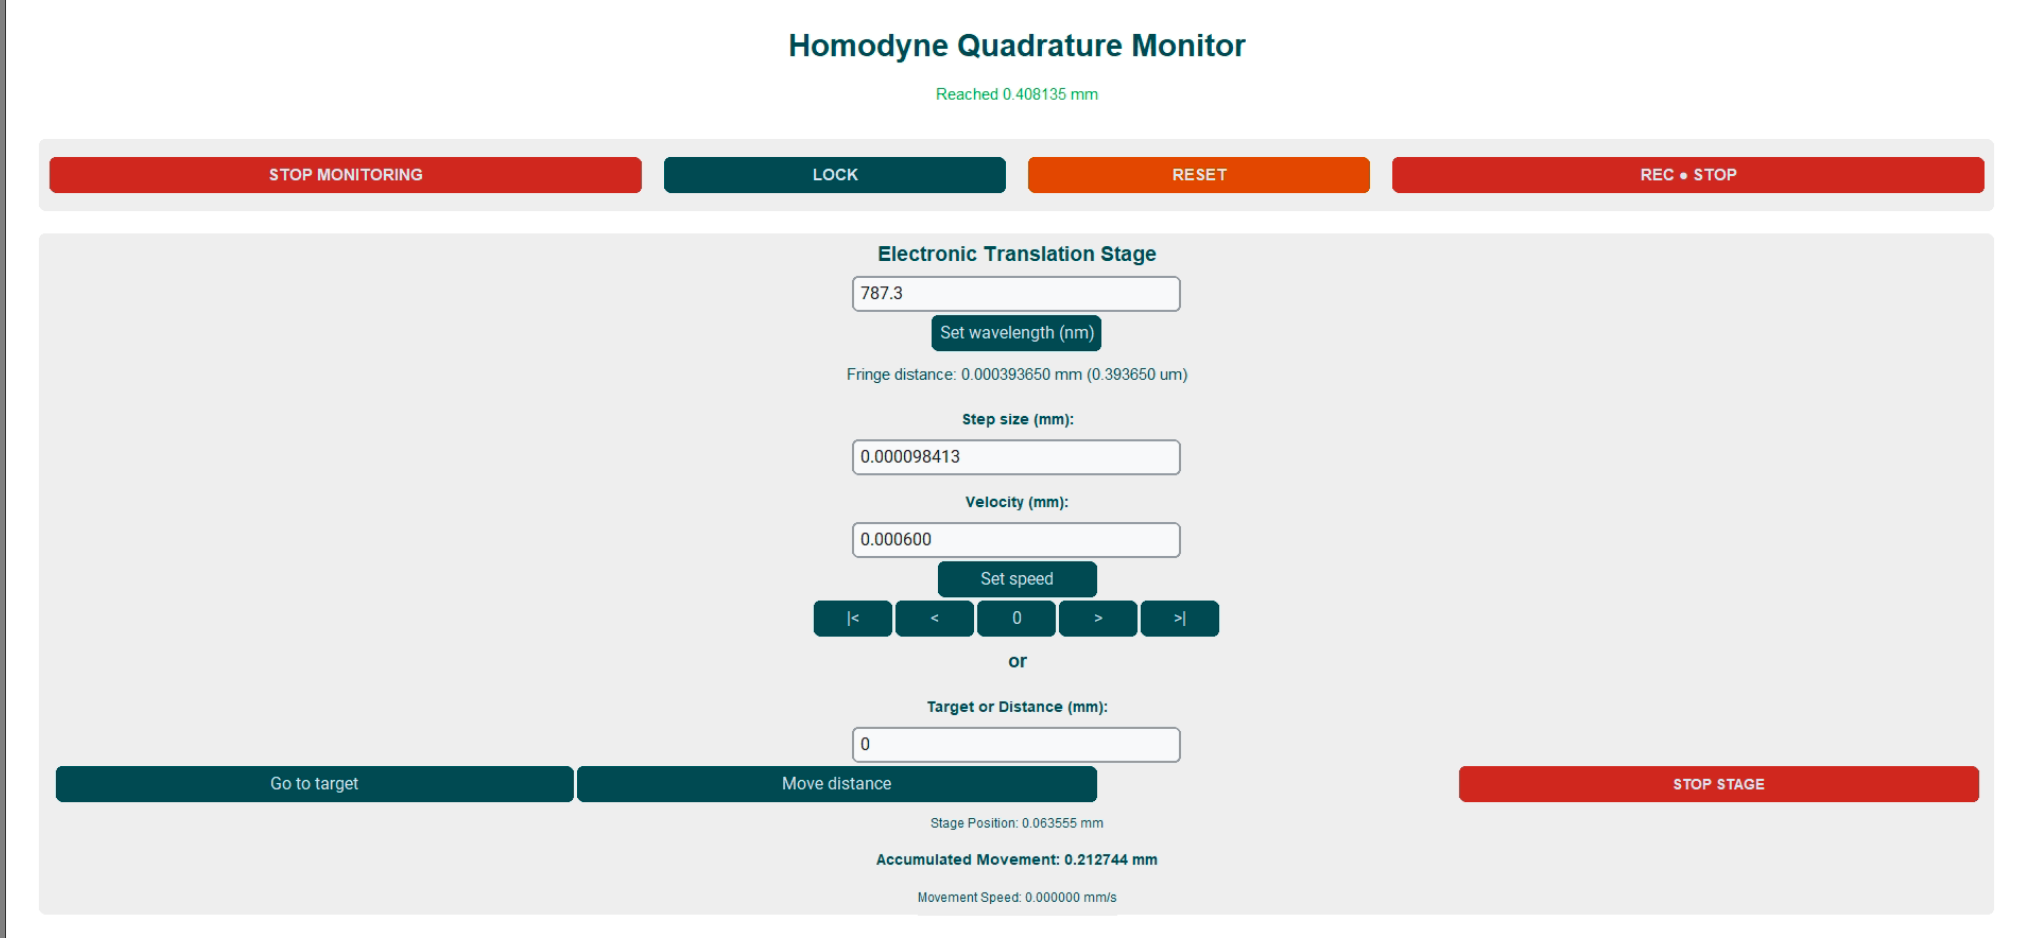
\includegraphics[width=0.92\linewidth]{figures/homodynesoftwareoben.png}\par\vspace{0.5em}
    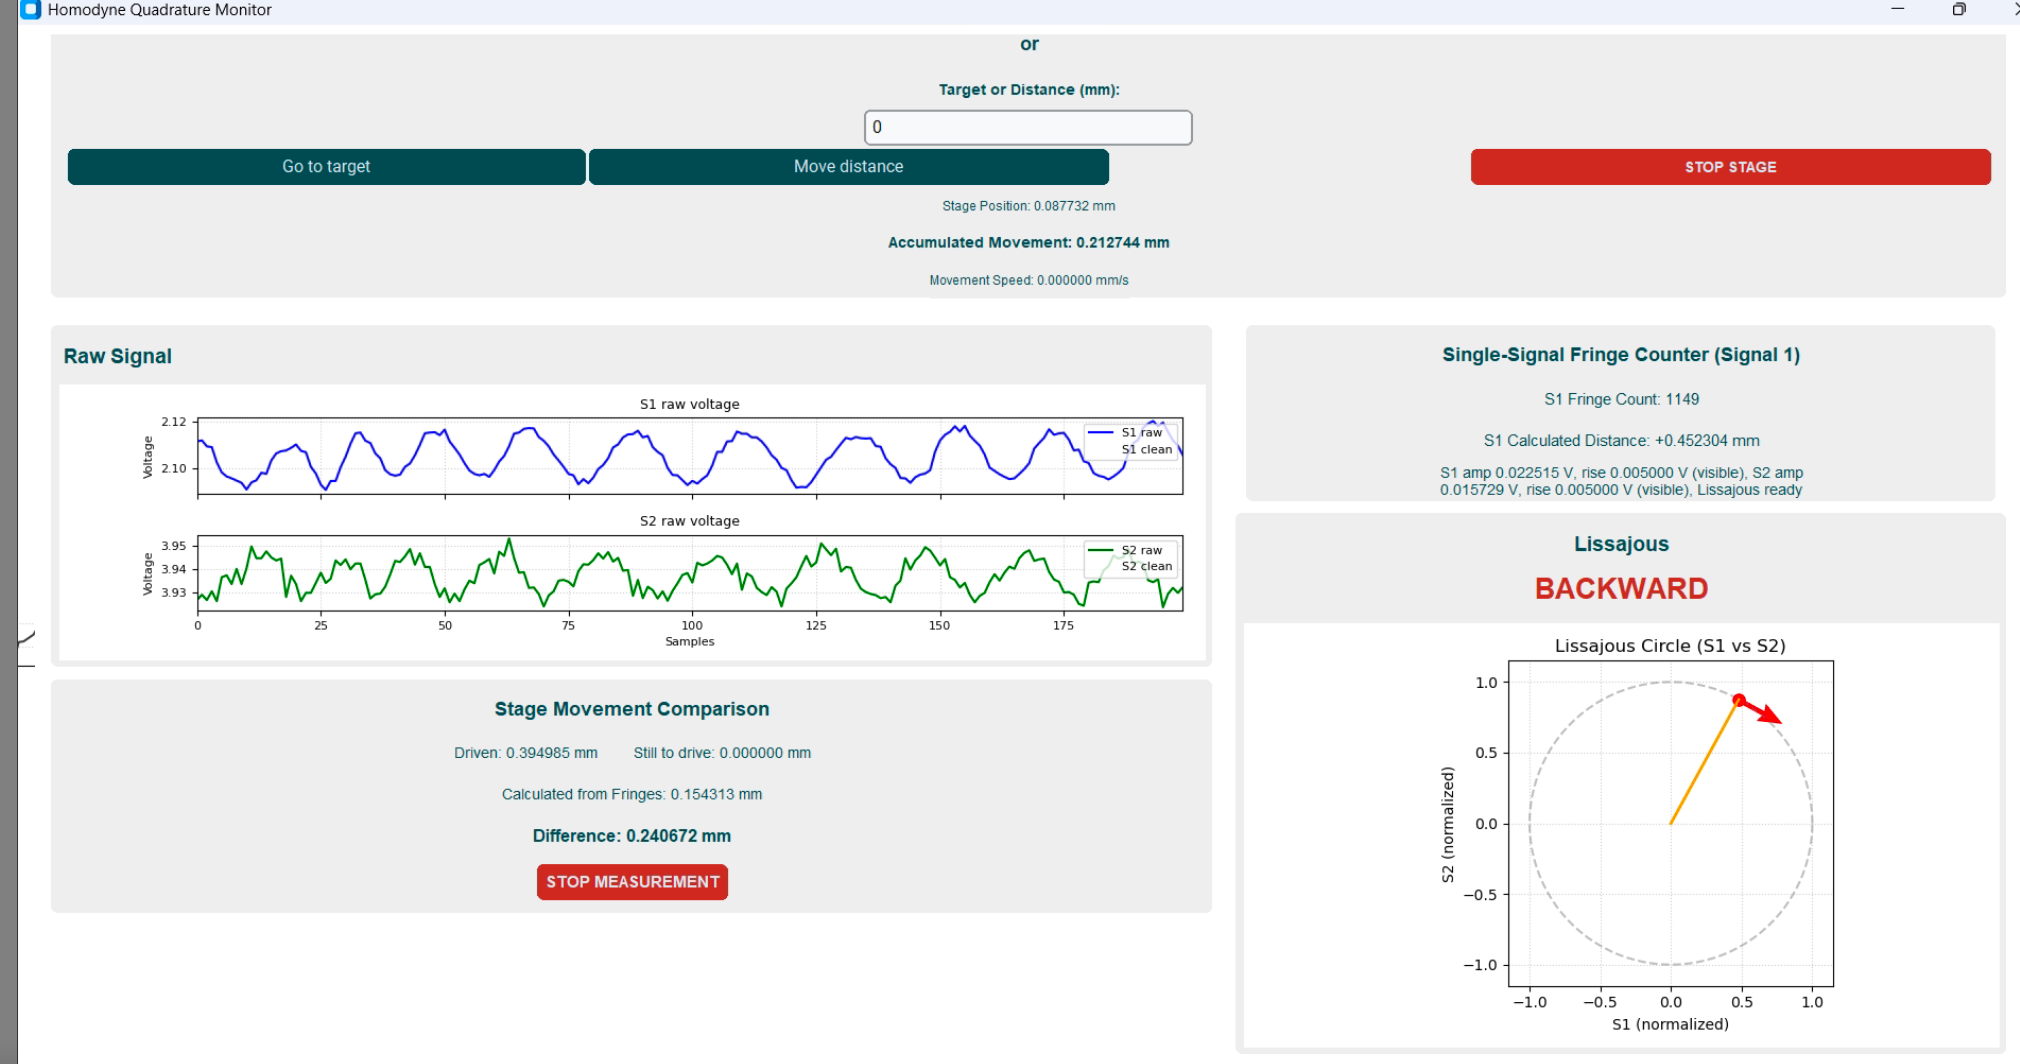
\includegraphics[width=0.92\linewidth]{figures/homodynesoftwareunten.png}
    \caption{Graphical user interface of the homodyne quadrature software. Top: upper part of the scrollable interface. Bottom: lower part of the interface.}
    \label{fig:homodyne_software_gui}
\end{figure}

\subsection{Calibration}

Before each measurement, both photodiode signals are calibrated. During this process, the translation stage is moved over a short distance while several interference fringes are recorded. From these measurements, the minimum and maximum voltages of each signal are determined. The voltage offset is calculated as

\begin{equation}
V_{\mathrm{offset}}=\frac{V_{\mathrm{max}}+V_{\mathrm{min}}}{2},
\end{equation}

while the normalization factor is given by

\begin{equation}
V_{\mathrm{scale}}=\frac{V_{\mathrm{max}}-V_{\mathrm{min}}}{2}.
\end{equation}

The normalized signals are then obtained by

\begin{equation}
S_{1,\mathrm{norm}}
=
\frac{S_1-V_{\mathrm{offset},1}}
{V_{\mathrm{scale},1}},
\end{equation}

\begin{equation}
S_{2,\mathrm{norm}}
=
\frac{S_2-V_{\mathrm{offset},2}}
{V_{\mathrm{scale},2}}.
\end{equation}

This normalization compensates for different signal amplitudes and voltage offsets of both photodiodes and approximately maps the measured data onto a unit circle in the Lissajous representation.

The fringe count is then detected using only one of the photodiodes and the exact same fringe counter as in the Single Photo diode software.

\subsection{Phase Determination}

The phase difference between the two normalized signals is calculated using the four-quadrant arctangent,

\begin{equation}
\varphi=\operatorname{atan2}
\left(
S_{2,\mathrm{norm}},
S_{1,\mathrm{norm}}
\right).
\end{equation}

\prismcite{39}. Since the arctangent only returns phase values between \(-\pi\) and \(\pi\), discontinuities occur whenever the phase crosses this interval. To obtain a continuous phase signal, phase unwrapping is necessary. The phase difference between two consecutive measurements is first wrapped back into the interval \([-\pi,\pi]\) and then accumulated,

\begin{equation}
\varphi_{\mathrm{unwrap}}
=
\varphi_{\mathrm{unwrap}}
+
\Delta\varphi.
\end{equation}

The accumulated phase is converted into the corresponding fringe position by

\begin{equation}
N_{\mathrm{fringe}}
=
\frac{\varphi_{\mathrm{unwrap}}}{2\pi}.
\end{equation}

Finally, the optical displacement is calculated using the fringe distance,

\begin{equation}
d
=
N_{\mathrm{fringe}}
\cdot
\frac{\lambda}{2},
\end{equation}

where \(\lambda\) is the laser wavelength.

\subsection{Direction Detection}


An advantage of the quadrature method is that the direction of movement can be determined directly from the sign of the phase change described in the previous section. To reduce the influence of noise, the software evaluates the average phase change over several samples instead of using a single value. If this average value is larger than the switching threshold of \(0.003\,\mathrm{rad}\), the motion is classified as forward. If it is smaller than \(-0.003\,\mathrm{rad}\), the motion is classified as backward. For smaller absolute phase changes, the stage is treated as stationary.

A lower release threshold of \(0.001\,\mathrm{rad}\) prevents short noise spikes from causing rapid switching between forward, backward, and stationary states.

\subsection{Lissajous Representation}

To visualize the measurement, the normalized photodiode signals are displayed as a Lissajous figure. Ideally, both signals form a circular trajectory, where the angular position corresponds directly to the optical phase \prismcite{31}. During operation, the current measurement point, the recent trajectory and the detected direction of rotation are updated continuously.

Since the raw photodiode signals are affected by electrical noise, the displayed circle is additionally smoothed. For this purpose, the phase of the last measurement points is approximated by a linear fit. The fitted phase is then transformed back into sine and cosine functions, resulting in a smooth circular trajectory. 

\subsection{Position Lock}

One limitation of the translation stage used in this work was that it did not remain perfectly stationary after reaching the commanded position. Instead, small mechanical drifts around the target position were observed. To compensate for these drifts, an active position lock was implemented.

The position lock can only be activated when no measurement is running. Likewise, once the lock is active, measurement mode and manual stage movements are disabled to avoid conflicts between user commands and the feedback controller.

When the user activates the lock, the current optical phase and the current height of the fringe count is defined as the reference position. If a previous calibration has already been performed, for example during a measurement, the calibrated fringe amplitudes are reused. Otherwise, the software prompts the user to enter an expected fringe amplitude manually. This value is then used as the detection threshold.

During operation, the software continuously evaluates both the single-photodiode fringe counter and the homodyne phase measurement. A correction is only initiated if two conditions are fulfilled simultaneously. First, the detected fringe must exceed the calibrated fringe threshold to avoid false detections caused by noise. Second, the homodyne evaluation must provide a valid movement direction. Only when both criteria are satisfied is the detected displacement interpreted as a real drift of the interferometer.

The required correction distance is calculated from the number of detected fringes and the corresponding fringe spacing. The translation stage is then commanded to move by the same distance in the opposite direction, thereby compensating the measured drift and returning the optical path length towards the reference position.

In practice, however, the achievable locking performance is limited by the mechanical behaviour of the translation stage. During every correction movement, additional interference fringes are generated because the stage itself is moving. These fringes are detected by the software and may trigger further correction movements before the previous correction has completely settled. Consequently, successive corrections are initiated although the original disturbance has already been compensated. With the positioning accuracy and response time of the available translation stage, this behaviour could not be completely eliminated. Therefore, the implemented position lock demonstrates the general feedback concept, but its long-term stability remains limited by the mechanical characteristics of the stage.

\subsection{Software Optimizations}

Due to the increasing number of implemented features, the computational workload of the software also increased. As a result, the graphical user interface became progressively less responsive. Although this issue could not be eliminated completely, mainly because of the large amount of data that had to be processed and displayed simultaneously within a Tkinter-based interface, several optimizations were implemented to significantly improve the responsiveness of the software.

The most important optimization was the extensive use of multithreading. Time-consuming tasks were executed in separate background threads, allowing the graphical user interface to continue updating independently. In particular, communication with the NI-DAQ device and the translation stage involves blocking hardware operations, which would otherwise freeze the user interface while waiting for a response. Therefore, all measurement routines, stage movements and hardware communication were executed in dedicated background threads, while the main thread was reserved exclusively for updating the graphical interface and processing user input.

The photodiode signals are sampled every

\begin{equation}
\Delta t_{\mathrm{sample}} = 5~\mathrm{ms},
\end{equation}

which corresponds to a sampling frequency of

\begin{equation}
f_{\mathrm{sample}} = 200~\mathrm{Hz}.
\end{equation}

This sampling rate was found to provide sufficient temporal resolution for fringe detection while keeping the computational load low.

Updating every graphical element at the sampling rate would unnecessarily increase the CPU usage and noticeably reduce the responsiveness of the interface. Therefore, the measurement thread only stores the newest acquired sample, while the graphical user interface is refreshed independently every

\begin{equation}
\Delta t_{\mathrm{UI}} = 100~\mathrm{ms},
\end{equation}

corresponding to an update frequency of

\begin{equation}
f_{\mathrm{UI}} = 10~\mathrm{Hz}.
\end{equation}


For the live voltage plots, only the most recent 200 samples are displayed. At a sampling frequency of \(200~\mathrm{Hz}\), this corresponds to a visible time window of approximately

\begin{equation}
T_{\mathrm{plot}}
=
200 \cdot 5~\mathrm{ms}
=
1~\mathrm{s}.
\end{equation}

The movement status of the translation stage is updated every

\begin{equation}
\Delta t_{\mathrm{stage}} = 100~\mathrm{ms},
\end{equation}

which is sufficient because the mechanical motion of the stage is several orders of magnitude slower than the photodiode sampling. During continuous stage movements, the position and velocity are recalculated every \(50~\mathrm{ms}\), providing smooth feedback without overloading the communication interface.

To further reduce computational effort, the live display is updated using a buffering mechanism. Newly acquired samples are stored temporarily and only the most recent sample is transferred to the graphical interface during the next scheduled update. Consequently, multiple measurement samples can be acquired between two graphical updates without increasing the frequency.